\documentclass[a4paper]{article}

\usepackage[T1]{fontenc}
\usepackage[utf8]{inputenc}
\usepackage{graphicx}
\usepackage{color}
\usepackage[intlimits]{amsmath}
\usepackage{amsfonts}
\usepackage{listings}
\usepackage{float}
\usepackage{setspace}
\usepackage[english]{babel}
\usepackage{fancyhdr}
\usepackage{booktabs}
\usepackage{multirow}
\usepackage{lastpage}
\usepackage[arrowmos]{circuitikz}
\usepackage[nottoc]{tocbibind}
\usepackage{url}
\usepackage[ugly]{units}
\usepackage[left=1.5cm,top=2cm,right=1.5cm,bottom=2.5cm]{geometry}
\usepackage[pdftex]{hyperref}
\usetikzlibrary{patterns,decorations.pathreplacing,automata,positioning,shapes,arrows}
\usepackage[T1]{fontenc}
%\usepackage{libertine}
\renewcommand*\oldstylenums[1]{{\fontfamily{fxlj}\selectfont #1}}
\setcounter{secnumdepth}{0}

\DeclareMathOperator{\ld}{ld}

\onehalfspacing
\setlength{\parindent}{0pt}

%\widowpenalty=1000
%\clubpenalty=1000

\tocsection

\author{Mathias Plichta}

\begin{document}
	\pdfinfo
	{/Creator (Mathias Plichta)
	 /Producer (pdflatex)
	 /Author (Mathias Plichta)
	}

\pagestyle{fancy}
\fancyhead{}
\fancyfoot{}
\renewcommand{\headrulewidth}{0pt}
\setlength{\parskip}{6pt}
\renewcommand{\headrulewidth}{.4pt}
\fancyhead[r]{Mathias Plichta, group 3}
\fancyhead[c]{Projektpraktikum IC-Entwurf}
\fancyhead[l]{Technische Universität München}
\fancyfoot[c]{Seite \thepage\ von \pageref{LastPage}}

\section{Display Driver}

\subsection{Overview}

The display driver translates character data into the signals required to
control the display. It also generates the sequence required to initialize the
display.

\begin{figure}
	\begin{center}
		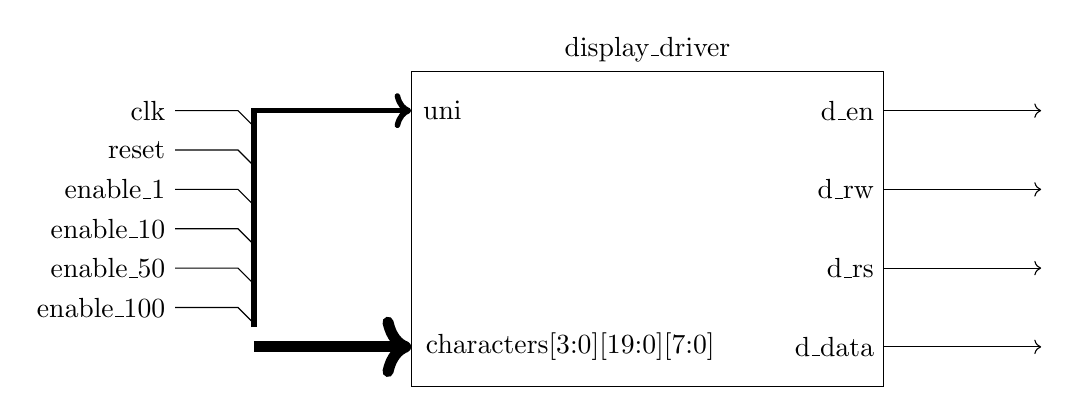
\begin{tikzpicture}
			%\draw[help lines] (-2, -6) grid (4, 2);

			\node[above] at (3,0) {display\_driver};

			\draw[line width=2pt,->] (-2, -3.25) |- (0, -0.5) node[right] { uni };

			\draw (-2, -0.5) ++(0,-.2) -- ++(-.2,.2) -- ++(-.8, 0) node[left] {clk};
			\draw (-2, -1.0) ++(0,-.2) -- ++(-.2,.2) -- ++(-.8, 0) node[left] {reset};
			\draw (-2, -1.5) ++(0,-.2) -- ++(-.2,.2) -- ++(-.8, 0) node[left] {enable\_1};
			\draw (-2, -2.0) ++(0,-.2) -- ++(-.2,.2) -- ++(-.8, 0) node[left] {enable\_10};
			\draw (-2, -2.5) ++(0,-.2) -- ++(-.2,.2) -- ++(-.8, 0) node[left] {enable\_50};
			\draw (-2, -3.0) ++(0,-.2) -- ++(-.2,.2) -- ++(-.8, 0) node[left] {enable\_100};

			\draw[line width=4pt,->] (-2, -3.5) -- (0, -3.5) node[right] { characters[3:0][19:0][7:0] };

			\draw[->] (6,-0.5) node[left] {d\_en}   -- ++(2, 0);
			\draw[->] (6,-1.5) node[left] {d\_rw}   -- ++(2, 0);
			\draw[->] (6,-2.5) node[left] {d\_rs}   -- ++(2, 0);
			\draw[->] (6,-3.5) node[left] {d\_data} -- ++(2, 0);

			\draw (0,0) rectangle (6, -4);
		\end{tikzpicture}
	\end{center}
	\caption{Block diagram of the display driver}
\end{figure}

To keep things simple, the display driver takes its input as a large array
which represents each character (\unit[8]{bit}) for each column and row of the
display. The Xilinx toolchain should be able to optimize away redundant logic
(for example characters that are always spaces or bit 7 of each character,
which is always 0).

Apart from the character array and the universal signals (\texttt{clk},
\texttt{reset}, \texttt{enable\_*}), no inputs are required. The three control
and eight data lines used to control the display are provided as outputs.

The display is refreshed periodically at a frequency of \unit[40.65]{Hz}, which
is sufficiently fast for the clock application. It is also much faster than the
time required for the display's pixels to completely transition between two
states.

\subsection{Implementation}

The display driver can be divided into three major parts (see figure~\ref{display_driver_impl}):

\begin{itemize}
	\item a shift register, which can load two display lines at a time and
	      convert them to a serial data stream. Includes a multiplexer to select
	      between both pairs of display lines, an enable input and a load input.
	\item Bus FSM: generates the \texttt{d\_e} signal (part of the display bus)
	      and \texttt{txdone}, which acts as an enable signal for the other
	      synchronous components. Its states are outlined in
	      figure~\ref{display_driver_bus}.
	\item Refresh FSM: generates the \texttt{d\_data} and \texttt{d\_rs} signals
	      that alternate between control commands and actual data. Its states
	      are outlined in figure~\ref{display_driver_refresh}.
\end{itemize}

\begin{figure}
	\begin{center}
		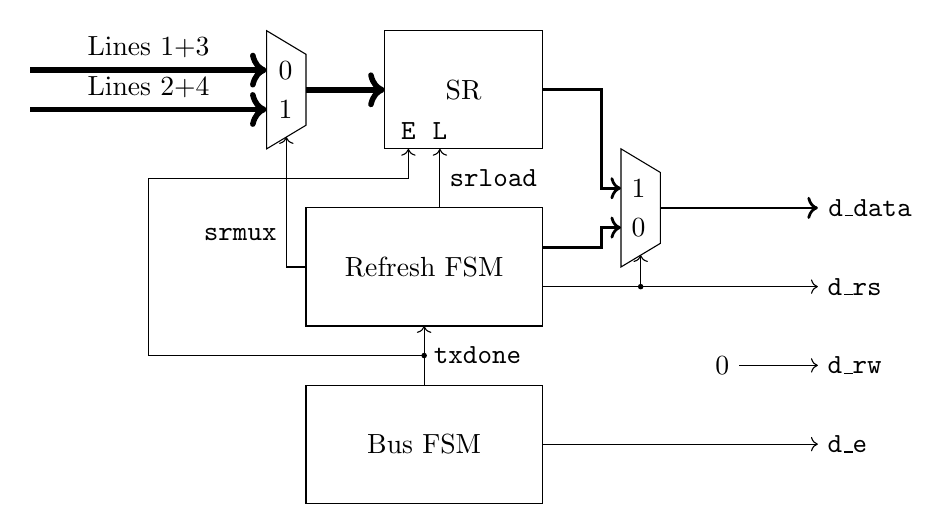
\begin{tikzpicture}
			\draw[line width=2pt,->] (0,0) -> (3, 0) node[midway,above] {Lines 1+3} node[right] {0};
			\draw[line width=2pt,->] (0,-.5) -> (3, -.5) node[midway,above] {Lines 2+4} node[right] {1};
			\draw[line width=2pt,->] (3.5,-.25) -> (4.5,-.25);
			\draw[line width=1pt,->] (6.5,-.25) -- (7.25,-.25) -- (7.25,-1.5) -> (7.5,-1.5) node[right] {1};
			\draw[line width=1pt,->] (6.5,-2.25) -- (7.25,-2.25) -- (7.25,-2) -> (7.5,-2) node[right] {0};
			\draw[line width=1pt,->] (8,-1.75) -> (10,-1.75) node[right] {\tt d\_data};

			\draw (3,.5) -- (3.5,.2) -- (3.5,-.7) -- (3,-1) -- cycle;

			\node at (5.5, -.25) {SR};
			\draw (4.5,.5) rectangle (6.5,-1);

			\node at(5,-2.5) {Refresh FSM};
			\draw (3.5,-1.75) rectangle (6.5,-3.25);

			\node at(5,-4.75) {Bus FSM};
			\draw (3.5,-4) rectangle (6.5,-5.5);

			\draw[->] (5,-4) -> (5,-3.25) node[right,midway] {\tt txdone};
			\draw[->] (5,-3.625) -- (1.5,-3.625) -- (1.5,-1.375) -- (4.8, -1.375) -> (4.8, -1) node[above] { \tt E };
			\fill (5,-3.625) circle (1pt);

			\draw[->] (3.5,-2.5) -- (3.25,-2.5) -> (3.25,-.85) node[left,near start] {\tt srmux};

			\draw[->] (5.2,-1.75) -> (5.2,-1) node[above] {\tt L} node[midway,right] {\tt srload};

			\draw (7.5,-1.0) -- (8,-1.3) -- (8,-2.2) -- (7.5,-2.5) -- cycle;

			\draw[->] (6.5,-2.75) -> (10,-2.75) node[right] {\tt d\_rs};
			\draw[->] (7.75,-2.75) -> (7.75,-2.35);
			\fill (7.75,-2.75) circle (1pt);
			\draw[->] (6.5,-4.75) -> (10,-4.75) node[right] {\tt d\_e};
			\draw[->] (9,-3.75) node[left] {0} -> (10,-3.75) node[right] {\tt d\_rw};
		\end{tikzpicture}
	\end{center}
	\caption{Display driver implementation overview}
	\label{display_driver_impl}
\end{figure}

\begin{figure}
	\begin{center}
		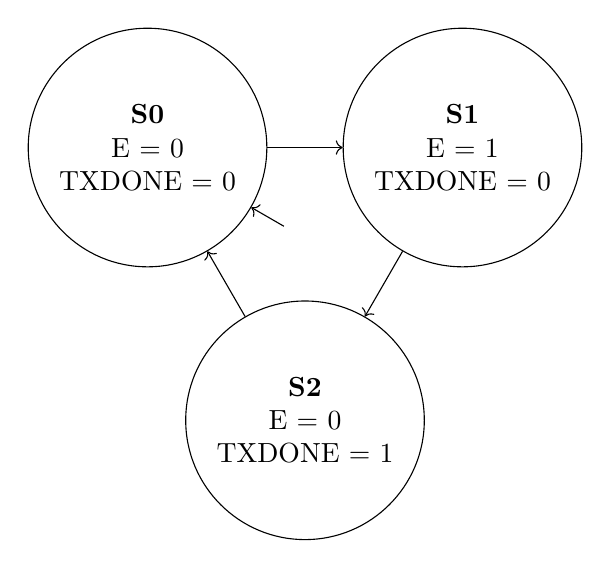
\begin{tikzpicture}[every state/.style={text width=2.5cm,align=center,node distance=.5cm},auto]
			\node[state] (S0) at (0.0,0) { \textbf{S0} \\ E = 0 \\ TXDONE = 0 };
			\node[state] (S1) at (4.0,0) { \textbf{S1} \\ E = 1 \\ TXDONE = 0 };
			\node[state] (S2) at (-60:4) { \textbf{S2} \\ E = 0 \\ TXDONE = 1 };

			\path[->] (S0) edge (S1)
						 (S1) edge (S2)
						 (S2) edge (S0)
						 (S0) ++ (-30:2) edge (S0);
		\end{tikzpicture}
	\end{center}
	\caption{Bus FSM: all transitions occur on CLK$\uparrow$}
	\label{display_driver_bus}
\end{figure}

\begin{figure}
	\begin{center}
		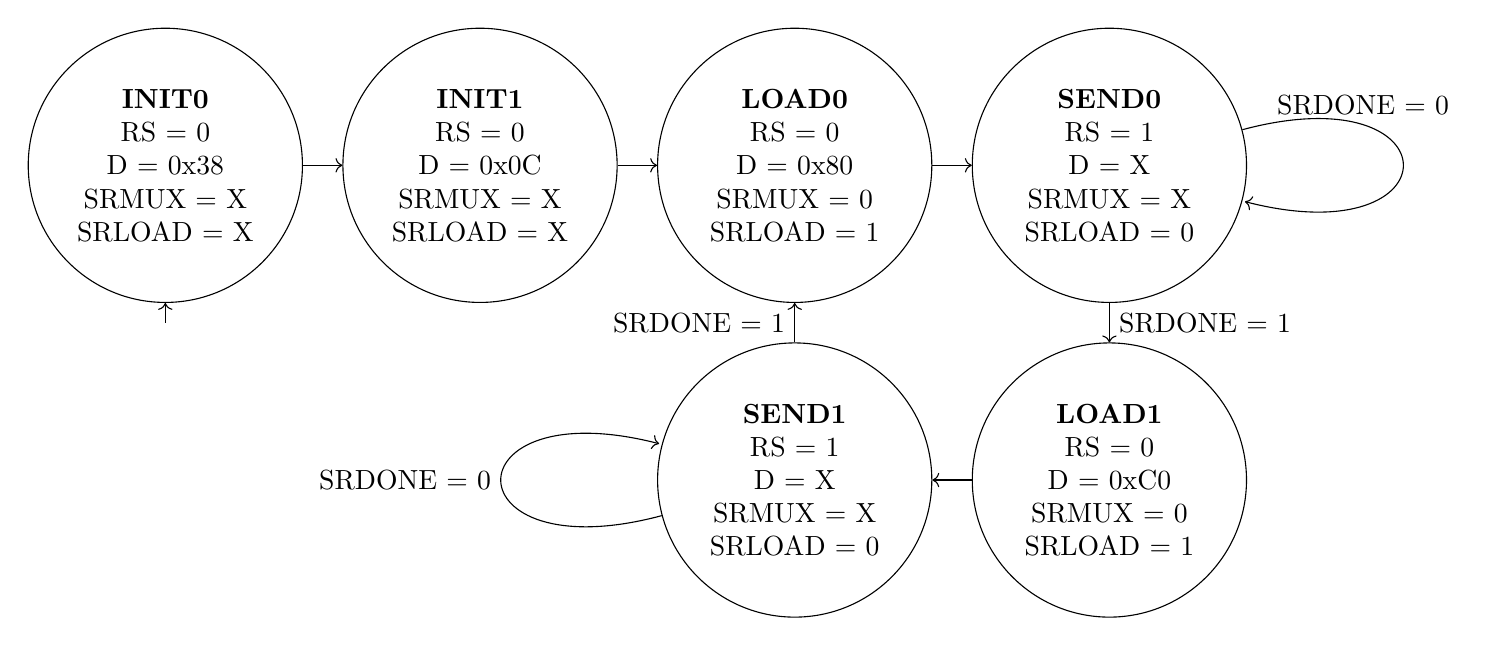
\begin{tikzpicture}[every state/.style={text width=2.5cm,align=center,node distance=.5cm},auto]
			\node[state]                       (FunctionSet)  { \textbf{INIT0} \\ RS = 0 \\ D = 0x38 \\ SRMUX = X \\ SRLOAD = X };
			\node[state,right=of FunctionSet]  (DisplayOnOff) { \textbf{INIT1} \\ RS = 0 \\ D = 0x0C \\ SRMUX = X \\ SRLOAD = X };
			\node[state,right=of DisplayOnOff] (SetAddrUpper) { \textbf{LOAD0} \\ RS = 0 \\ D = 0x80 \\ SRMUX = 0 \\ SRLOAD = 1 };
			\node[state,right=of SetAddrUpper] (WriteUpper)   { \textbf{SEND0} \\ RS = 1 \\ D = X    \\ SRMUX = X \\ SRLOAD = 0 };
			\node[state,below=of WriteUpper]   (SetAddrLower) { \textbf{LOAD1} \\ RS = 0 \\ D = 0xC0 \\ SRMUX = 0 \\ SRLOAD = 1 };
			\node[state,left =of SetAddrLower] (WriteLower)   { \textbf{SEND1} \\ RS = 1 \\ D = X    \\ SRMUX = X \\ SRLOAD = 0 };

			\path[->] (FunctionSet) ++(0,-2) edge (FunctionSet)
						 (FunctionSet)  edge                                  (DisplayOnOff)
						 (DisplayOnOff) edge                                  (SetAddrUpper)
						 (SetAddrUpper) edge                                  (WriteUpper)
						 (WriteUpper)   edge             node {SRDONE = 1}    (SetAddrLower)
											 edge[loop right,near start,above] node {SRDONE = 0} ()
						 (SetAddrLower) edge                                  (WriteLower)
						 (WriteLower)   edge             node {SRDONE = 1}    (SetAddrUpper)
											 edge[loop left]  node {SRDONE = 0}    ();
		\end{tikzpicture}
	\end{center}
	\caption{Refresh FSM: all transitions occur on CLK$\uparrow$ if TXDONE = 1}
	\label{display_driver_refresh}
\end{figure}

\subsection{Testing Strategy}

The unit was tested against a behavioral implementation of the display itself,
which verifies reception of the correct initialization and address commands and
outputs the received display contents as an array. This array is then compared
to the input of the display driver module under test.

The testbench also verifies timing constraints using the minimum delays given
in the display datasheet. An example waveform can be seen in
figure~\ref{display_driver_waveform}.

\begin{figure}
	\begin{center}
		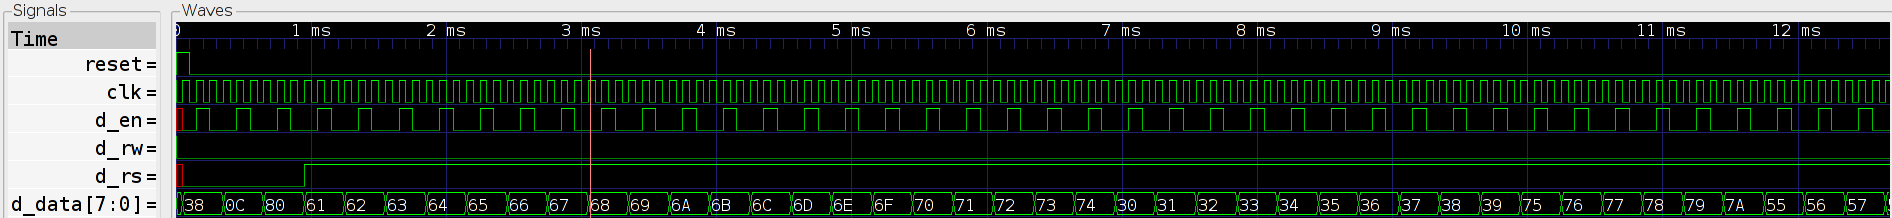
\includegraphics[width=\textwidth]{display_driver_timing_reset.png}
	\end{center}
	\caption{Simulated output of the display driver}
	\label{display_driver_waveform}
\end{figure}

\section{Time buffer}

\subsection{Overview}

\begin{figure}
	\begin{center}
		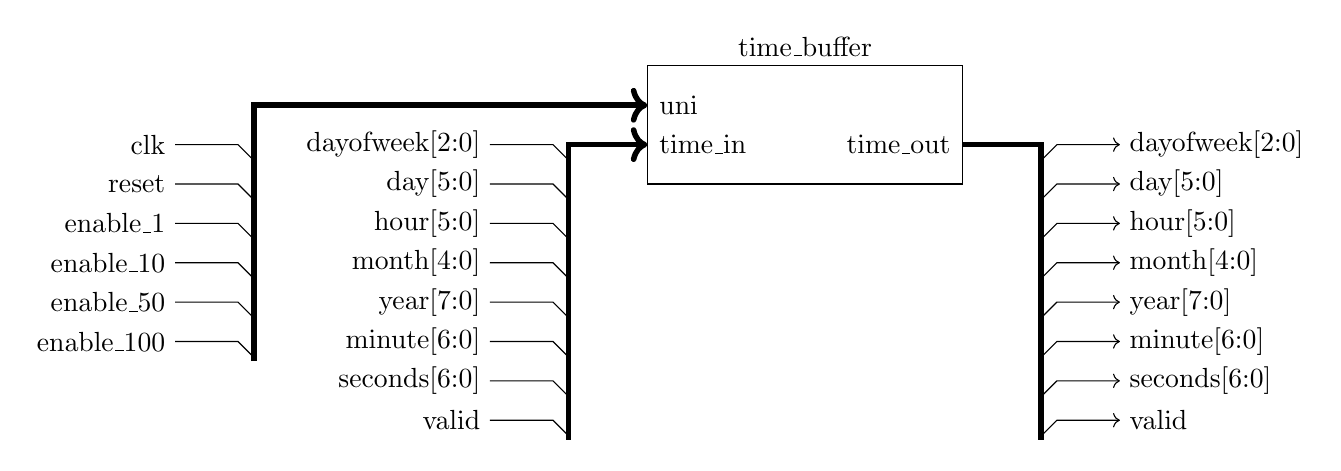
\begin{tikzpicture}
			%\draw[help lines] (-2, -6) grid (4, 2);

			\node[above] at (2,0) {time\_buffer};

			\draw[line width=2pt,->] (-5, -3.75) |- (0, -0.5) node[right] { uni };

			\draw (-5, -1.0) ++(0,-.2) -- ++(-.2,.2) -- ++(-.8, 0) node[left] {clk};
			\draw (-5, -1.5) ++(0,-.2) -- ++(-.2,.2) -- ++(-.8, 0) node[left] {reset};
			\draw (-5, -2.0) ++(0,-.2) -- ++(-.2,.2) -- ++(-.8, 0) node[left] {enable\_1};
			\draw (-5, -2.5) ++(0,-.2) -- ++(-.2,.2) -- ++(-.8, 0) node[left] {enable\_10};
			\draw (-5, -3.0) ++(0,-.2) -- ++(-.2,.2) -- ++(-.8, 0) node[left] {enable\_50};
			\draw (-5, -3.5) ++(0,-.2) -- ++(-.2,.2) -- ++(-.8, 0) node[left] {enable\_100};

			\draw[line width=2pt,->] (-1, -4.75) |- (0, -1.0) node[right] { time\_in };

			\draw (-1, -1.0) ++(0,-.2) -- ++(-.2,.2) -- ++(-.8, 0) node[left] {dayofweek[2:0]};
			\draw (-1, -1.5) ++(0,-.2) -- ++(-.2,.2) -- ++(-.8, 0) node[left] {day[5:0]};
			\draw (-1, -2.0) ++(0,-.2) -- ++(-.2,.2) -- ++(-.8, 0) node[left] {hour[5:0]};
			\draw (-1, -2.5) ++(0,-.2) -- ++(-.2,.2) -- ++(-.8, 0) node[left] {month[4:0]};
			\draw (-1, -3.0) ++(0,-.2) -- ++(-.2,.2) -- ++(-.8, 0) node[left] {year[7:0]};
			\draw (-1, -3.5) ++(0,-.2) -- ++(-.2,.2) -- ++(-.8, 0) node[left] {minute[6:0]};
			\draw (-1, -4.0) ++(0,-.2) -- ++(-.2,.2) -- ++(-.8, 0) node[left] {seconds[6:0]};
			\draw (-1, -4.5) ++(0,-.2) -- ++(-.2,.2) -- ++(-.8, 0) node[left] {valid};

			\draw[line width=2pt] (5, -4.75) |- (4, -1.0) node[left] { time\_out };

			\draw[->] (5, -1.0) ++(0,-.2) -- ++(.2,.2) -- ++(.8, 0) node[right] {dayofweek[2:0]};
			\draw[->] (5, -1.5) ++(0,-.2) -- ++(.2,.2) -- ++(.8, 0) node[right] {day[5:0]};
			\draw[->] (5, -2.0) ++(0,-.2) -- ++(.2,.2) -- ++(.8, 0) node[right] {hour[5:0]};
			\draw[->] (5, -2.5) ++(0,-.2) -- ++(.2,.2) -- ++(.8, 0) node[right] {month[4:0]};
			\draw[->] (5, -3.0) ++(0,-.2) -- ++(.2,.2) -- ++(.8, 0) node[right] {year[7:0]};
			\draw[->] (5, -3.5) ++(0,-.2) -- ++(.2,.2) -- ++(.8, 0) node[right] {minute[6:0]};
			\draw[->] (5, -4.0) ++(0,-.2) -- ++(.2,.2) -- ++(.8, 0) node[right] {seconds[6:0]};
			\draw[->] (5, -4.5) ++(0,-.2) -- ++(.2,.2) -- ++(.8, 0) node[right] {valid};

			\draw (0,0) rectangle (4, -1.5);
		\end{tikzpicture}
	\end{center}
	\caption{Block diagram of the time buffer}
\end{figure}

The time buffer receives the decoded DCT signal (including the valid bit and a
seconds field which will always be zero). If the valid bit is set, it buffers
the time and valid bit in an internal register. Every full second after a reset
or received valid signal, the stored time is incremented. If an increment
causes the seconds to overflow from 59 back to 0, the stored valid bit is
reset.

At reset, the stored time is set to Sat January 1, 2000, 00:00:00 and marked as
invalid.

\subsection{Implementation}

A simple asynchronous ripple carry adder is used to compute the value of the
currently stored time plus one second. Some simple logic is used to generate
carry/reset signals at the borders between BCD digits (for example, both digits
of the hour field are reset and the day is incremented iff the previous value
of the hour field was 23 and its carry-in was set).

Similarily, asynchronous logic determines the number of days in the current
month based on the month and year fields, so the overflow from day to month can
be handled correctly.

A counter is used to count the clock ticks that passed since the last update of
the date/time register, and the appropriate action is taken based on this
counter and the values of the valid and reset inputs.

\subsection{Testing strategy}

Since there are so many special cases to be considered when dealing with time
and date arithmetic, a test bench was created that prints out the current time
once per simulated second. It will either leave the unit alone, yieling one
line per second, or permanently set the hours, minutes and seconds to 23:59:59,
allowing fast testing of the date logic.

Both versions of the test bench were run to create one secondly log file
containing a couple of days' worth of data, and one daily log file containing
all dates in the 21st century. A simple PHP script was written to create the
same data using PHP's built-in time and date functions, and the results were
compared using the UNIX diff tool.

\end{document}
